\documentclass[a4paper,10pt]{article}
\usepackage{graphicx,wrapfig,hyperref}
\usepackage[hmargin=3.5cm,vmargin=3.0cm]{geometry}
\begin{document}

\title{TI2800 Contextproject - My Cultural Heritage\\ Architectural Design}
\author{Sjoerd van Bekhoven\\ Tim Eversdijk \\ Herman Blanken \\ Rutger Plak \and 4014774 \\ 4005562 \\ 4078624 \\ 1358375}

\newcommand{\itemb}[1]{\item \textbf{#1}}

\maketitle
\renewcommand*\contentsname{Inhoudsopgave}

\thispagestyle{empty}
\vspace{10cm}
		\begin{figure}[ht!]
				\centering
				
\includegraphics[width=\textwidth]{cultuurapp-logo.png}
			\end{figure}
\clearpage
\setcounter{page}{0} 
\thispagestyle{empty} 
\ 
\clearpage
\tableofcontents
\clearpage


\section{Introductie}
In dit document wordt de structuur van de software, bestaande uit verschillende softwarecomponenten uitgewerkt. De relaties tussen deze componenten, communicatie tussen deze componenten en de eigenschappen van deze componenten worden gegeven. Dit gebeurt aan de hand van de externe kenmerken van de verschillende softwarecomponenten.

	\subsection{Doel van het systeem}
	Het systeem heeft als doel om gebruikers de mogelijkheid te geven:
	\begin{itemize}
		\item Monumenten te zoeken en deze met elkaar te vergelijken. [Req:3.2]
		\item Monumenten met een categorisch of visuele gelijkenis moeten ontdekt kunnen worden. [Req:3.13\&3.14]
		\item Daarnaast moet het mogelijk zijn om in de buurt van een bepaald monument te zoeken naar faciliteiten als caf\'eís, restaurants e.d..[Req:3.6]
	\end{itemize}
	
	\subsection{Definities, acroniemen en afkortingen}
		\subsubsection{Afkortingen}
		\begin{tabular}{ l | l }
			DB & Database \\
			HTML & Hyper Text Markup Language \\
			ext4 & Fourth Extended File System \\
			PHP & Pre- Hypertext Processor \\
			SQL & Structured Query Language \\
			XML & Extended Markup Language
		\end{tabular}
	
		\subsubsection{Definities}
		\begin{tabular}{ l | l }
			Client & Een computerssysteem dat toegang heeft tot de\\& webserver van CultuurApp. \\
			(CultuurApp-)User/Gebruiker & Een gebruiker van de CultuurApp.\\
Toerist & Een anonieme bezoeker van de CultuurApp.
		\end{tabular}
		
	\subsection{Referenties}
	\begin{itemize}
		\item Context Project Guideline - Blackboard
		\item Object-Orientated Software Engineering - Timothy C. Lethbridge Robert Lagani\`ere.
	\end{itemize}
	
\section{Voorgestelde software architectuur}
Het systeem bestaat op het hoogste niveau uit drie delen. In dit hoofdstuk wordt per onderdeel toegelicht welke taken dit deel heeft en waar het weer uit bestaat. Voor het overzicht van het hele diagram zie appendix A figuur \ref{componentdiagramoverview}.

	\subsection{Ontwerppatroon}
	\begin{itemize}
		\itemb{HMVC} 
Het systeem wordt ontwikkeld volgens een HMVC-patroon. Dit staat voor een Hierarchical-Model-View-Controller-patroon. Kohana\footnote{http://kohanaframework.org/}, een PHP-framework, maakt gebruik van dit patroon en het CultuurApp-systeem bouwt daar op voort. Een HMVC-patroon schrijft voor dat de modellen (de daadwerkelijke data), de weergave en de controllers in gescheiden bestanden en mappen worden geprogrammeerd. Op deze manier is het terugvinden van specifieke code makkelijker en de code zelf blijft ook overzichtelijker. In het CultuurApp-systeem worden de modellen en controllers zelfs volledig gescheiden van de views daar de views op de client worden opgebouwd.
		\begin{figure}[ht!]
		\centering
		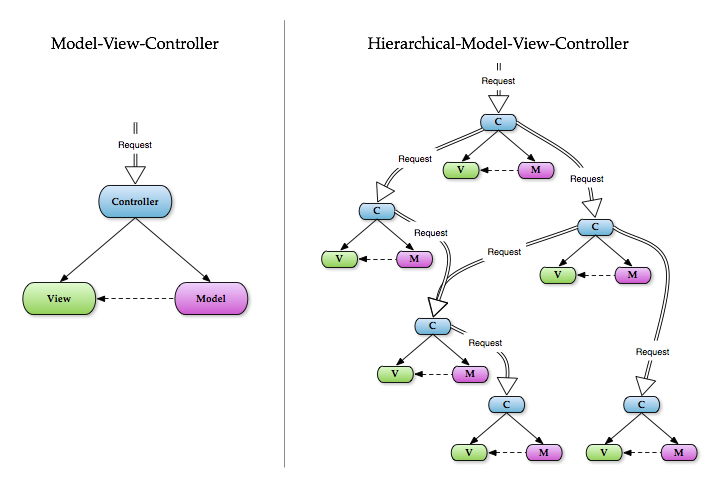
\includegraphics[width=12cm]{MVC-HMVC.png}
		\caption{\label{hmvc}HMVC, bron ibuildings.com\footnote{http://techportal.ibuildings.com/2010/02/22/scaling-web-applications-with-hmvc/}}
		\end{figure}
	
\itemb{Client-server model}
		Door veel javascript te gebruiken aan de kant van de client, wordt veel rekenwerk van de server verplaatst naar de kant van de client. Dit ontlast de server. Externe foto's worden niet gedownload maar de locatie van de afbeelding wordt slechts doorgegeven aan de client. De javascript op de client side zorgt voor de afhandeling en het downloaden van de afbeelding. Dit mindert het dataverkeer van de server.
	
\itemb{Pipe-and-filter model}
		Image processing wordt op drie processing units synchroon uitgevoerd. Deze informatie wordt gecombineerd. Deze drie processing units verdelen de belasting. Er worden voor de image processing nauwelijks webserver-resources gebruikt, slechts voor het downloaden van de locaties van de afbeeldingen en het uploaden van de resultaten van de image processing.
	\end{itemize}

	\subsection{Ontwerpprincipes}
		\begin{enumerate}
			\itemb{Divide and conquer}
			Om iedere database-tabel komt een PHP-klasse. Door de verschillende componenten in de database onder te verdelen in verschillende klassen, blijft de ORM Factory overzichtelijk en zijn de verschillende klassen onafhankelijk van elkaar te ontwikkelen. Voor iedere externe databron bestaan aparte harvesters. Deze verschillende harvesters zorgen ervoor dat onafhankelijke databronnen elkaar niet in de weg zitten. Tevens kunnen de harvesters onafhankelijk van elkaar ontwikkeld worden.
					 	 	 		
\itemb{Reduce coupling where possible}
Tussen externa databronnen en de rest van het systeem zitten harvesters. Door gebruik van deze harvesters kunnen eventuele fouten in de externe data worden afgevangen en is de rest van het systeem niet afhankelijk van de externe databronnen omdat de harvesters altijd een verwacht antwoord kunnen geven.

\itemb{Increase reusability where possible}
Door tussen de database en de verschillende gebruikers van data uit de database een ORM factory te cre\"eeren kunnen (nog) niet bestaande componenten eenvoudig deze ORM factory gebruiken om data uit de database te halen. Aan de hand van deze API het eenvoudig om het systeem te gebruiken of uit te breiden.

\itemb{Design for flexibility}
Door op de zojuist beschreven manier data van datagebruikende scripts te scheiden kunnen componenten op een flexibele manier, zonder dat andere componenten daar last van hebben, aangepast worden.

\itemb{Design for testability}
Voor de implementatie wordt gestart worden voor elke methode sluitende test-cases geschreven.
		\end{enumerate}

	\subsection{Systeemcomponenten (figuur \ref{componentdiagramhighlevel})}
	\begin{itemize}
		\item Front-end $\Rightarrow$ Draait op Javascript op de computer / handheld van de gebruiker van het systeem.
		\item Back-end $\Rightarrow$ Debian server waarop PHP en MySQL draaien.
		\item Processing-end $\Rightarrow$ Dit deel van het systeem verwerkt de afbeeldingen uit de data-set en upload deze naar de back-end. De processing vindt plaats op aparte machines, onafhankelijk van de server voor de back-end.
		\item External Sources $\Rightarrow$ Externe servers, zoals die van Google en Facebook. [Req:3.1.1 \& 3.4 \& 3.5 \& 3.6 \& 3.8 \& 3.9]

	\end{itemize}
	\begin{figure}[ht!]
	\centering
	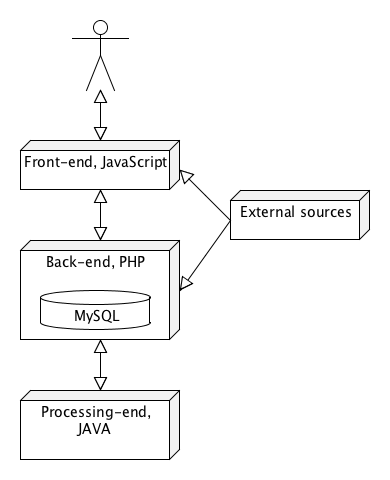
\includegraphics[width=8cm]{componentDiagram_highlevel.png}
	\caption{High Level Component Diagram \label{componentdiagramhighlevel}}
	\end{figure}
	
	\subsection{Subsysteem decompositie}
		\subsubsection{Javascript front-end (figuur \ref{componentdiagramfrontend})}
		\begin{itemize}
			\item Templater $\Rightarrow$ Combineert HTML en data om een view te cre\"eeren voor de gebruiker.
			\item Combiner $\Rightarrow$ Combineert data uit verschillende externe sources.
			\item Login form $\Rightarrow$ Post data naar de server om authenticatie uit te voeren.
		\end{itemize}

		\begin{figure}[ht!]
		\centering
		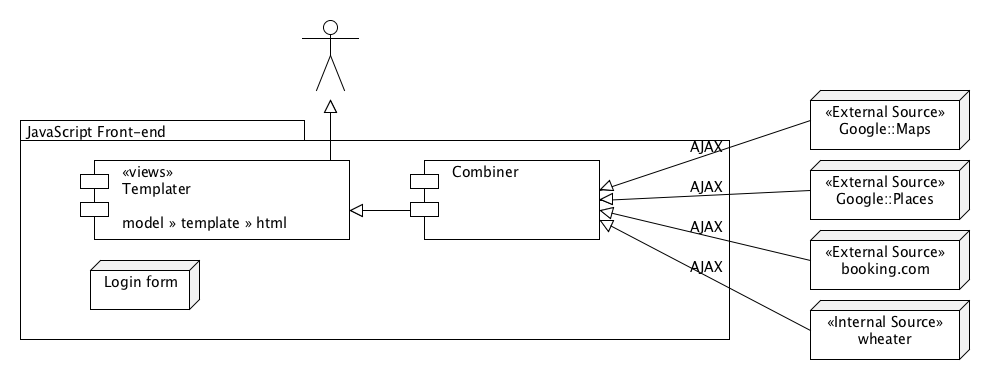
\includegraphics[width=14cm]{componentDiagram_frontend.png}
		\caption{Component Diagram Javascript Front-end \label{componentdiagramfrontend}}
		\end{figure}
	
		\subsubsection{PHP back-end}
		\begin{itemize}
			\item Users (zie figuur \ref{componentdiagramuser}) $\Rightarrow$ De identiy-combiner zorgt ervoor dat facebook en OpenID [Req:3.9]
 gekoppeld kan worden aan de gebruikers van het systeem. De acties van de gebruiker worden opgeslagen in de database door de Logger.
				\begin{figure}[ht!]
				\centering
				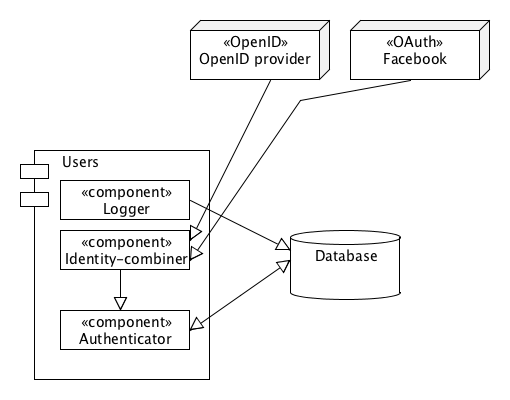
\includegraphics[width=8.5cm]{componentDiagram_user.png}
				\caption{Component Diagram Users \label{componentdiagramuser}}
				\end{figure}
			
			\item ORMfactory (zie figuur \ref{componentdiagramanalysis}) $\Rightarrow$ Alle communicatie tussen PHP en de database in de vorm van objecten zal plaats vinden in de ORMfactory.
			\item Textual-linker (zie figuur \ref{componentdiagramanalysis}) $\Rightarrow$ tekstuele vergelijkingen maken met gebruik van tags, omschrijvingen en een thesaurus [Req:3.14]. Hiervan wordt gebruikgemaakt bij het zoeken naar relevante fotoís op Flickr.
			\item User-profiler (zie figuur \ref{componentdiagramanalysis}) $\Rightarrow$ plaatst gebruikers in een bepaalde groep door analyse van de opgeslagen logs en social-media profiel [Req:3.12].
				\begin{figure}[ht!]
				\centering
				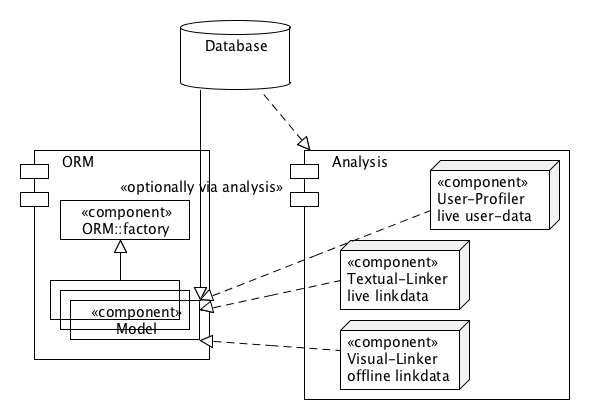
\includegraphics[width=8.5cm]{componentDiagram_analysis.png}
				\caption{Component Diagram Analysis \label{componentdiagramanalysis}}
				\end{figure}
			\item Harvesters (zie figuur \ref{componentdiagramharvesters}) $\Rightarrow$
				\begin{itemize}
					\item Flickr-harvester $\Rightarrow$ datacommunicatie met Flickr [Req:3.8].
					\item 4SQ-harvester $\Rightarrow$ datacommunicatie met Foursquare [Req:3.4].
					\item Weather-dataharvester $\Rightarrow$ datacommunicatie met Wunderground [Req:3.5]. 
				\end{itemize}
				\begin{figure}[ht!]
				\centering
				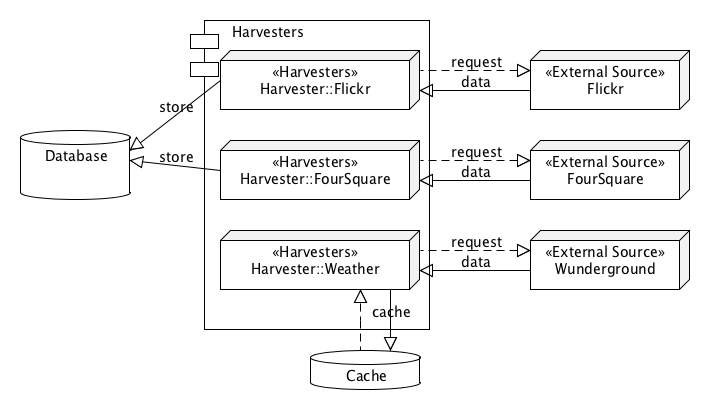
\includegraphics[width=10cm]{componentDiagram_harvesters.png}
				\caption{Component Diagram Harvesters \label{componentdiagramharvesters}}
				\end{figure}
			\item Database $\Rightarrow$ opslag van data.	
		\end{itemize}
		
		\subsubsection{Java / Compiled back-end (figuur \ref{componentdiagramprocessing})}
			\begin{itemize}
				\item Java / Image $\Rightarrow$ Vergelijken van afbeeldingen uit de database.Hiervan wordt gebruikgemaakt bij het completeren van de dataset en het vergelijken van monumenten [Req:3.13].
				\item PC-Processing Unit (x3) $\Rightarrow$ Machines waarop de java applicaties draaien.
			\end{itemize}
				\begin{figure}[ht!]
				\centering
				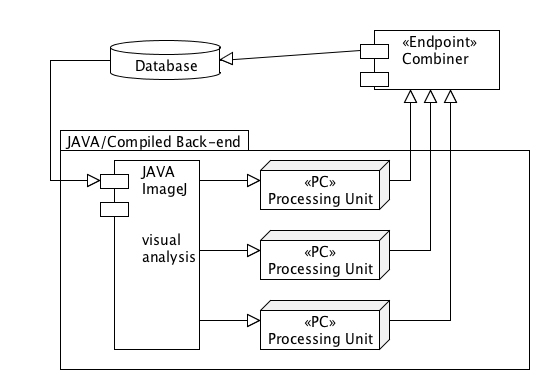
\includegraphics[width=10cm]{componentDiagram_processing.png}
				\caption{Component Diagram Java / Compiled back-end \label{componentdiagramprocessing}}
				\end{figure}
		
	\subsection{Hardware/Software mapping (figuur \ref{hardwarediagram})}
	De webserver zal bestaan uit \'e\'en machine met Apache en MySQL. Image-processing [Req:3.13] gebeurt op drie externe machines (Processing Units). Vanuit diverse externe databronnen wordt extra informatie gehaald. De informatie zal aan de kant van de gebruiker van het systeem op zijn webbrowser of handheld getoond worden [Req\#56].
	\begin{figure}[ht!]
	\centering
	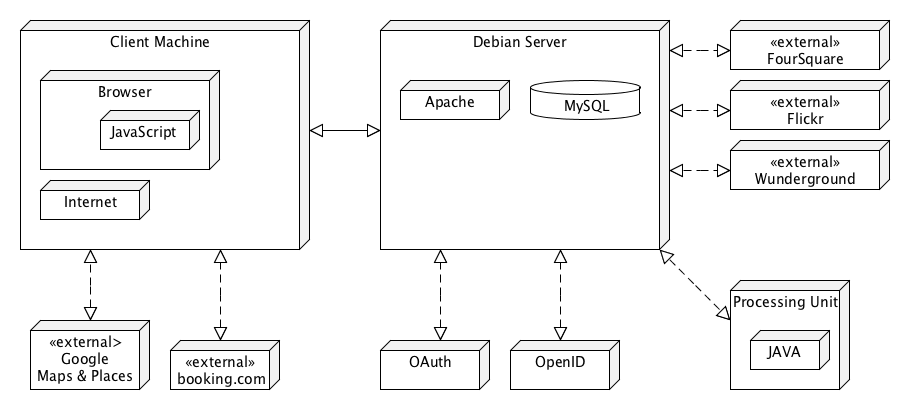
\includegraphics[width=15cm]{hardwareDiagram.png}
	\caption{Hardware Diagram \label{hardwarediagram}}
	\end{figure}
	
	\subsection{Persistent Data Management}
	Fotoís van externe bronnen worden niet opgeslagen, enkel een kleine versie wordt lokaal opgeslagen [Req\#31]. De ge\"uploade foto's [Req\#36] worden wel lokaal op het ext4 bestandsysteem van de Debian server bewaard. De data-set die is aangeleverd door de opdrachtgever wordt opgeslagen in de database. Ook wanneer van externe bronnen data wordt opgehaald - zoals van FourSquare, Twitter en Flickr - wordt deze data opgeslagen [Req:3.4].\\ \\
De persoongegevens van gebruikers worden na opvragen van de authenticatie provider opgeslagen in de database. Meerdere identiteiten (van verschillende providers) kunnen worden gekoppeld aan \'e\'en gebruiker [Req\#32\&33].
	\begin{figure}[ht!]
	\centering
	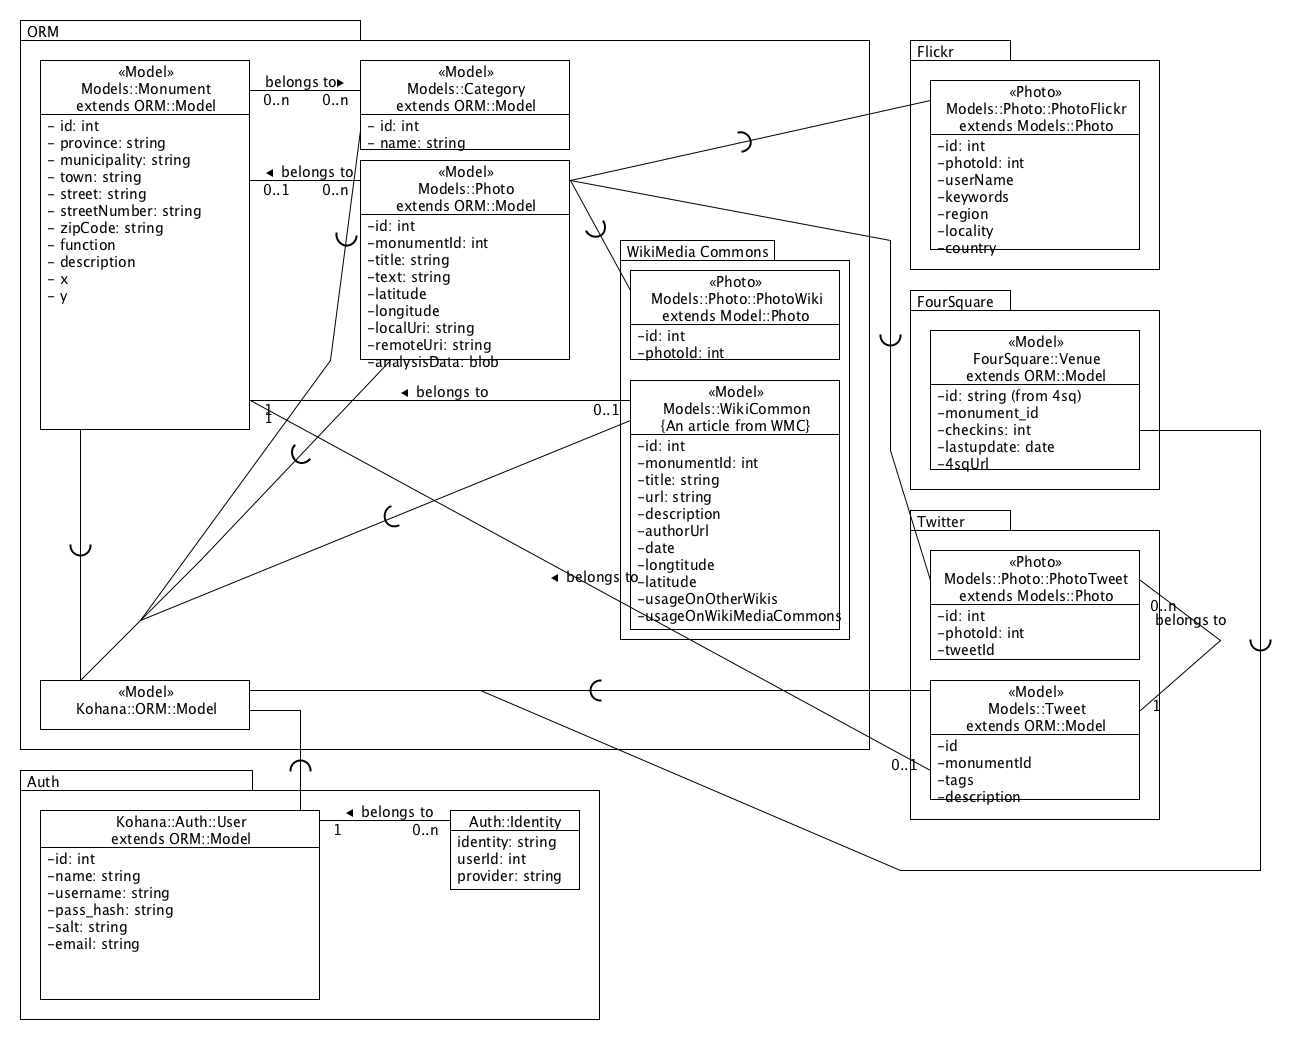
\includegraphics[width=15cm]{entityRelationshipDiagram.png}
	\caption{Entity Relation Diagram \label{entityrelationshipdiagram}}
	\end{figure}

	\subsection{Global Resource Handling en Access Control voor verschillende actoren}
	Het systeem bestaat uit drie delen waarvan twee op systemen draaien op beheerde machines. De back-end zal continue data moeten kunnen leveren. Omdat MySQL schaalbaar is en het systeem op meerdere machines kan tegelijk draaien is het mogelijk om zeer grote pieken op te vangen met meerdere servers. Bij de ontwikkeling van het systeem wordt er echter vanuit gegaan dat er met \'e\'en server genoeg gebruikers kunnen worden bediend.\\ \\
De machines voor processing verwerken data onafhankelijk van de back-end en zijn niet gevoelig voor pieken in de bezoekersaantallen. Bij de initi\"ele verwerking van de data-set zullen veel resources (werkgeheugen en opslag) en processorkracht nodig zijn, hiervoor zullen meerdere machines worden gebruikt. Later is een enkele machine genoeg om de toegevoegde data te verwerken [Req\#54\&47].\\ \\
Soorten actoren:
	\begin{itemize}
		\item Toerist (anonieme gebruiker)
		\item CultuurApp-gebruiker (ingelogde gebruikers)
	\end{itemize}

Wanneer de gebruikers bij het systeem zijn ingelogd kunnen ze content toevoegen, anonieme gebruikers kunnen dit niet. Bij het toevoegen van data wordt gecontroleerd of er een gebruiker is ingelogd, zo niet dan lukt het toevoegen niet en zal de gebruiker eerst worden gevraagd in te loggen via een van de vele beschreven authenticatie providers [Req:3.9].

	\subsection{Concurrency}
		\subsubsection{Websitebezoek}
		Wanneer een gebruiker het systeem gebruikt zal deze diverse aanroepen naar de PHP back-end doen. De PHP back-end zal vervolgens weer gebruik maken van de database. De front-end draait bij de systeemgebruiker op zijn handheld / computer.
		
		\subsubsection{Image-processing}
		De machines voor image-processing draaien enkele keren per dag, wanneer er nieuwe data is om te verwerken [Req\#47]. 
		
		\subsubsection{Back-up}
		Aangezien het systeem vooral Nederlandse gebruikers zal hebben zullen de pieken in de bezoekersaantallen vooral overdag voorkomen (+1 GMT). ës Nachts zal de server veelal idle zijn en kan er dan ge-back-upt worden zonder dat de server daar hinder van ondervindt. Wanneer het systeem in productie gaat is het slim om te kijken op welke momenten er weinig bezoekers zijn. De back-ups kunnen het beste in deze dalen van bezoekersaantallen gemaakt worden. [Req\#71]
		
		\subsubsection{Harvesting}
		De harvesters zullen niet continu data ophalen van de externe bronnen. Specifieke data kan worden opgevraagd wanneer een bezoeker deze aanvraagt, algemene updates van de content worden echter uitgevoerd aan de hand van een planning. Afhankelijk van hoe hoog de druk op de server is zal het vergaren van data worden uitgesteld of eerder worden ingepland. De individuele gebruiker kan een algehele harvest niet starten.
	
	\subsection{Randvoorwaarden}
		\subsubsection{Back-end}
		\textit{Users (figuur \ref{componentdiagramuser}, pagina \pageref{componentdiagramuser})} \\
		Het authenticatie gedeelte van het gebruikers-systeem zou kunnen crashen/falen als de service van OpenID, Facebook of onze eigen inlog service wegvalt [Req:3.9]. In dit geval valt automatisch ook het gebruiker specifieke logging gedeelte uit en word er alleen nog maar gelogd voor anonieme gebruikers [Req\#46]. Ook zullen alle gebruikers specifieke services zoals favorieten [Req:3.11] en profiel gerelateerde voorkeuren [Req:3.17] niet gebruikt kunnen worden. Dit is dus niet echt een essentieel component omdat het grootste gedeelte van het systeem het nog gewoon naar behoren doet.\\ 
		\\ \textit{Database} \\
		Mocht de ORMfactory of de Database uitvallen is het niet meer mogelijk data op te halen of op te slaan en doet het hele systeem het niet meer. Dit zijn dus erg essenti\"ele componenten. Wel blijft de front-end gewoon draaien welke in de huis-stijl een foutmelding zal weergeven.\\ 
		\\ \textit{Harvesters (figuur \ref{componentdiagramharvesters}, pagina \pageref{componentdiagramuser})} \\
		Voor alle vier de harvesters geldt dat ze niet heel essentieel zijn voor het systeem en er prima even uit kunnen liggen. Sommige data is dan tijdelijk niet beschikbaar maar het systeem blijft gewoon naar behoren werken. De harvesters zouden er bijvoorbeeld uit kunnen liggen als een van onze externe data sources offline is. In de praktijk zal dit echter zelden gebeuren.
		
		\subsubsection{Front-end}
		\textit{Javascript (figuur \ref{componentdiagramfrontend}, pagina \pageref{componentdiagramfrontend})} \\
		Mocht javascript bij de client niet werken werkt onze hele front-end niet. Deze kan dan namelijk niet communiceren met onze back-end. Het is dus erg essentieel dat javascript wel werkt bij de client. Dit is over het algemeen wel het geval.
		\subsubsection{Java / Compiled back-end}
		\textit{Image-processing (PC-Processing Unit) (figuur \ref{componentdiagramprocessing}, pagina \pageref{componentdiagramprocessing})} \\
		Visuele kenmerken plaatjes construeren. Dit is geen kritiek proces. Om de zoveel tijd zal er offline een analyse gemaakt worden van images en aan het systeem worden toegevoegd. Dit systeem kan dus niet uitvallen omdat het niet standaard draait.	
	
		\clearpage

\appendix
	\section{Component Diagram} \label{sec:appendix1}
	\begin{figure}[ht!]
		\centering
		
\includegraphics[width=\textwidth]{componentDiagram.png}
		\caption{Component Diagram \label{componentdiagramoverview}}
	\end{figure}

\end{document}